\begin{ledgroupsized}[r]{120mm}
\footnotesize 
\pstart 
\noindent\textbf{\"{U}berlieferung:}
\pend
\end{ledgroupsized} 
%
\begin{ledgroupsized}[r]{114mm}
\footnotesize 
\pstart \parindent -6mm
\makebox[6mm][l]{\textit{L}}Aufzeichnung: LH XXXVII 5 Bl. 201, 204. 1 Bog. 2\textsuperscript{o}. 1 S. auf Bl. 204~v\textsuperscript{o}. Bl. 204~r\textsuperscript{o} ist leer. Bl. 201 überliefert N. 19. % F/1 = 037,05_201
Der Bog. umschließt ferner Bl. 202-203 (N. 21). \\% F/3 = 037,05_202-203
% Wasserzeichen auf Bl. 201.
Cc 2, Nr. 971 B
\pend
\end{ledgroupsized}
%
\vspace*{5mm}
\begin{ledgroup}
\footnotesize 
\pstart
\noindent\footnotesize{\textbf{Datierungsgr\"{u}nde}: Das vorliegende Stück N. 20 % F/2 = 037,05_204
befindet sich auf demselben Textträger wie das Stück N.~19
 % F/1 = 037,05_201
und weist auch inhaltlich einen engen Zusammennhang mit diesem letzteren auf. Aus diesen Gründen wird für das vorliegende Stück die für N. 19 % F/1 = 037,05_201
vorgeschlagene Datierung übernommen.}
\pend
\end{ledgroup}
%
\vspace*{8mm}
\count\Afootins=1200
\count\Bfootins=1200
\count\Cfootins=1200
\pstart 
\noindent
\normalsize
[204~v\textsuperscript{o}] Resistentia Trabis\protect\index{Sachverzeichnis}{resistentia trabis} eadem est, sive rumpatur in $C$ sive
\edtext{in $D$. Ponamus}{\lemma{in $D$.}\Bfootnote{\textit{(1)}\ Ergo p \textit{(2)}\ Ponamus \textit{L}}}
eam
\edtext{esse 12}{\lemma{esse}\Bfootnote{\textit{(1)}\ 8 \textit{(2)}\ 12 \textit{L}}}
\edtext{librarum,\protect\index{Sachverzeichnis}{libra} radio}{\lemma{librarum,}\Bfootnote{\textit{(1)}\ scilicet pond \textit{(2)}\ ex cen \textit{(3)}\ radio \textit{L}}}
assumto $CB$ vel $CA.$
ita enim tam pondus $E$ quam
\edtext{pondus\protect\index{Sachverzeichnis}{pondus} $F$ erit 6}{\lemma{pondus $F$}\Bfootnote{\textit{(1)}\ esse 4 \textit{(2)}\ erit 6 \textit{L}}}
librarum.
\pend
\pstart
Ponamus porro lineam $CB$ esse 4 ulnarum\protect\index{Sachverzeichnis}{ulna} lineam $AD$ esse
\edtext{[2]}{\lemma{}\Bfootnote{2 \textit{erg. Hrsg.}}}
ulnarum lineam $DB$ esse 6 ulnarum.
Pondus\protect\index{Sachverzeichnis}{pondus} \edtext{appensum ex}{\lemma{appensum}\Bfootnote{\textit{(1)}\ in \textit{(2)}\ ex \textit{L}}}
[$DB$]\edtext{}{\lemma{$DC$}\Bfootnote{\textit{L ändert Hrsg.}}}
\edtext{esto $h$.}{%
\lemma{esto $h$}\Cfootnote{Zur Bezeichnung von Gewichten verwendet Leibniz im Text, anders als in der Abbildung [\textit{Fig. 1}], sowohl Klein- als auch Großbuchstaben.}}
Potentia\protect\index{Sachverzeichnis}{potentia} ejus afficietur a brachio 6 ulnarum $DB$ ut potentia ponderis $f$ a brachio\protect\index{Sachverzeichnis}{brachium} 4 ulnarum\protect\index{Sachverzeichnis}{ulna} $CB$ ita ut si $f$ et $h$ ponerentur aequalia, per \edtext{se, potentia}{\lemma{se,}\Bfootnote{\textit{(1)}\ habitu \textit{(2)}\ potentia \textit{L}}} $h$ ad potentiam $f$ futura sit ut 6 \edtext{ad 4. Fingamus}{\lemma{ad 4.}\Bfootnote{\textit{(1)}\ Ponamus \textit{(2)}\ Fingamus \textit{L}}} pondus $h$ esse 
\pend
\vspace{2.0em}% PR: Rein provisorisch !!!
% \begin{wrapfigure}{l}{0.4\textwidth}
% \begin{center}
\pstart
\noindent
\centering
\setline{17}
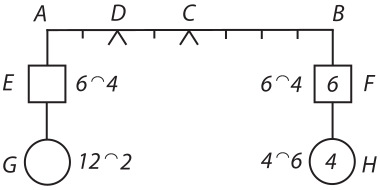
\includegraphics[width=0.452\textwidth]{images/lh03705_204v-d1.pdf}\\
\centering
%\vspace*{1.0em}
%\newline
%\rule{0mm}{0mm}\centering
[\textit{Fig. 1}]\edtext{}{\lemma{\hspace*{1,8mm}[\textit{Fig. 1}]}\killnumber\Cfootnote{\cite{00050}Vgl. die Abbildung in G. \textsc{Galilei}, \textit{Discorsi}, Leiden 1638, S. 136 (\cite{00048}\textit{GO} VIII, S. 176).}}
%\caption{Bildbeschreibung}
% \end{center}
%\end{wrapfigure}
\pend
%\vspace*{1.5em}% PR: Rein provisorisch !!!
\pstart
\noindent4 librarum eadem erit ipsius potentia quae est ponderis $f$ etsi \edtext{ex diversa distantia}{\lemma{ex}\Bfootnote{\textit{(1)}\ diverso loco, quia di \textit{(2)}\ diversa distantia \textit{L}}}
viribusque\protect\index{Sachverzeichnis}{vis} diversis, quia distantiae sunt in permutata ponderum ratione. At contra pondus $G$ debet esse gravius quam 4 in ea ratione, qua distantia est minor, ita cum distantia $AD$ sit dimidia distantiae $AC$ pondus erit \edtext{duplum, 12}{\lemma{duplum,}\Bfootnote{\textit{(1)}\ 8 \textit{(2)}\ 12 \textit{L}}} librarum,\protect\index{Sachverzeichnis}{libra}
ita enim pondus $G$ quoque ponderi\protect\index{Sachverzeichnis}{pondus}
[$E$]\edtext{}{\lemma{$G$}\Bfootnote{\textit{L ändert Hrsg.}}}
potentia\protect\index{Sachverzeichnis}{potentia} aequivalebit.
Ac proinde \edtext{cum potentia}{\lemma{cum}\Bfootnote{\textit{(1)}\ pondus \textit{(2)}\ potentia \textit{L}}} $G$ potentiae $E$ et potentia $H$ potentiae $F$ aequivaleant, \edtext{etiam summa potentiarum}{\lemma{etiam}\Bfootnote{\textit{(1)}\ potentiae \textit{(2)}\ summa \textit{(a)}\ potentiae \textit{(b)}\ potentiarum \textit{L}}} $G+H$ summae potentiarum $E+F$ aequivalebit, quod requirebatur. Potest tamen fieri ut summa potentiarum aequivaleant, etsi singulae non aequivaleant, dum altera alterius defectum compenset, et v.g. tanto major
\edtext{sit, ultra quam requirat locus, quanto}{\lemma{sit,}\Bfootnote{\textit{(1)}\ quanto \textit{(2)}\ ultra [...] quanto \textit{L}}}
altera minor, citra quam requirat locus.% \edtext{
% \newline
% \hspace*{7,5mm}
%Ut}{\lemma{}\Bfootnote{locus.\
% \textbar\
\pend
\vspace{1.5em}
\pstart
[\textit{Folgender kleingedruckter Text ist im Manuskript gestrichen}:]
\pend
\vspace{0.5em}
\pstart
\noindent
\footnotesize
% \hspace*{-2,5mm}
% \hspace*{-0,4mm}$\protect\begin{array}[b]{l}
$\displaystyle 6 \hspace{4,5mm} 2 \hspace{5,0mm} 6 \hspace{4,5mm} 6 \hspace{5,5mm} 6 \overgroup{\phantom{aic}} 2 \hspace{5,1mm} 6 \overgroup{\phantom{aic}} 6 \hspace{7,5mm} 12 \hspace{21,5mm} 12 \hspace{9,5mm} 36 \hspace{10,0mm} 36$
\newline%
$\displaystyle g\smallfrown AD + h \smallfrown DB = e \smallfrown AD + e \smallfrown DB = g \smallfrown AD + h \smallfrown DB - e \smallfrown AD = e \smallfrown DB - h \smallfrown DB.$
% \protect\end{array}$
\newline%
\noindent%
\rule[0mm]{0mm}{5mm}%
$\displaystyle g - e , \smallfrown AD = e - h \smallfrown \llcorner DB \lrcorner .$
\quad Ergo $\displaystyle g - e = e - h \smallfrown \frac{DB}{AD}.$
\quad Ergo $\displaystyle\frac{g-e}{e-h}=\frac{DB}{AD}.$
\newline%
\noindent%
\rule[-3,5mm]{0mm}{0mm}%
$\displaystyle g - e \smallfrown \cancel{AD} = e - h \smallfrown \frac{DB}{AD}.$
\newline%
\indent%
Nota si terminus alicujus sit 0 nulla est ejus ratio, quare hic cessat Analysis.
% \textit{gestr.}\
% \textbar\
\pend
\vspace{1.5em}
\pstart
Ut
% \textit{L}}}
pone
\edtext{pondus\protect\index{Sachverzeichnis}{pondus} $G$}{\lemma{pondus}\Bfootnote{\textit{(1)}\ $H$ \textit{(2)}\ $G$ \textit{L}}}
esse 6 librarum\protect\index{Sachverzeichnis}{libra} (cum debuerit esse 12).
Ejus potentia\protect\index{Sachverzeichnis}{potentia} erit $6 \smallfrown 2$
\edtext{$\displaystyle = 12$}{\lemma{$\displaystyle = 12$}\Bfootnote{\textit{erg. L}}} librarum
\edtext{cum debeat esse 24.}{\lemma{cum debeat esse 24}\Bfootnote{\textit{erg. L}}}
Debet ergo potentia ponderis $H$ esse librarum 36.
Et cum distantia ejus a centro sit 6 debet esse
\edtext{librarum 6. Observari potest}{\lemma{librarum}\Bfootnote{\textit{(1)}\ 9 \textit{(2)}\ 6. \textit{(a)}\ Ubi \textit{(b)}\ Unde sequitur \textit{(c)}\ Observari potest \textit{L}}}
elegans Corollarium eandem manere vim\protect\index{Sachverzeichnis}{vis rumpendi} \edtext{rumpendi}{\lemma{rumpendi}\Bfootnote{\textit{erg. L}}},
utcunque varietur fulcrum, ponderibus \edtext{invariatis, quod generaliter demonstrari potest}{\lemma{invariatis}\Bfootnote{\textit{(1)}\ . At pondera requirere \textit{(2)}\ , quod generaliter demonstrari potest \textit{L}}}.
At nunquam pondera\protect\index{Sachverzeichnis}{pondus} erunt sufficientia, \edtext{sed}{\lemma{sufficientia,}\Bfootnote{\textit{(1)}\ nisi \textit{(2)}\ sed \textit{L}}} vel justo majora, vel justo minora, nisi sint in permutata ratione \edtext{distantiarum}{\lemma{ratione}\Bfootnote{\textit{(1)}\ brachiorum\protect\index{Sachverzeichnis}{brachium} \textit{(2)}\ distantiarum \textit{L}\hspace{-3mm}}} a medio, etsi in eo non sit fulcrum.\protect\index{Sachverzeichnis}{fulcrum}
Sed elegantissima in hoc argumento propositio \edtext{haec est}{\lemma{propositio}\Bfootnote{\textit{(1)}\ est \textit{(2)}\ haec est \textit{L}\hspace{-3mm}}}: Differentia inter pondus \edtext{$G$}{\lemma{}\Bfootnote{$G$ \textit{erg. L}}} appensum ex loco propiori \edtext{$DA$}{\lemma{}\Bfootnote{$DA$ \textit{erg. L}\hspace{-3mm}}} hoc loco 12, et \edtext{pondus $E$ vel $F$}{\lemma{}\Bfootnote{pondus $E$ vel $F$ \textit{erg. L}}} appensum ex medio \edtext{$CB$}{\lemma{}\Bfootnote{$CB$ \textit{erg. L}}} hoc loco 6. quae differentia facit 6 \edtext{$(12-6)$}{\lemma{}\Bfootnote{$(12-6)$ \textit{erg. L}}}, esse ad differentiam inter pondus \edtext{$H$ 4}{\lemma{}\Bfootnote{$H$ 4 \textit{erg. L}}} appensum ex loco remotiori \edtext{$DB$}{\lemma{remotiori}\Bfootnote{\textit{(1)}\ hoc loco \textit{(2)}\ $DB$ \textit{L}}} et \edtext{dictum}{\lemma{}\Bfootnote{dictum \textit{erg. L}}} pondus $E$ vel $F$ appensum ex loco medio $CB$ quae differentia facit 2 \edtext{$(6-4)$}{\lemma{}\Bfootnote{$(6-4)$ \textit{erg. L}}} ac proinde 6 ad 2 esse ut distantia major $DB$ 6 ad minorem $AB$ 2, quod theorema hac aequatione exprimitur:
\rule[-4mm]{0mm}{10mm}$\displaystyle\frac{g-e}{e-h} = \frac{DB}{AD}$.
Quod quia inexpectatum est, videbantur enim prima fronte, pondera potius quam differentiae distantiis proportionales esse debere.
At vero exemplo ostendimus, pondera\protect\index{Sachverzeichnis}{pondus} posse esse distantiis minime proportionalia, sed aequalia inter se, etiam ex distantiis a fulcro diversis; et contra \edtext{differentias ponderum}{\lemma{differentias}\Bfootnote{\textit{(1)}\ ut \textit{(2)}\ ponderum \textit{L}}} inaequalium a \edtext{medio seu}{\lemma{medio}\Bfootnote{\textit{(1)}\ et \textit{(2)}\ seu \textit{L}}} uno aequalium esse distantiis proportionales, ut mox demonstrabimus; et pondera non esse \edtext{reciproce}{\lemma{}\Bfootnote{reciproce \textit{erg. L}}} proportionalia distantiis a fulcro, \edtext{sed a medio}{\lemma{sed a}\Bfootnote{\textit{(1)}\ pondere \textit{(2)}\ medio \textit{L}}}, ubicunque sit fulcrum. Sed ad haec demonstranda, nos ita praeparabimus: atque ideo eandem virium summam\protect\index{Sachverzeichnis}{summa virium} in iis variato utcunque fulcro\protect\index{Sachverzeichnis}{fulcrum} manere.
\pend
\count\Afootins=1500
\count\Bfootins=1500
\count\Cfootins=1500